
%\documentclass[aspectratio=169]{beamer}
\documentclass{beamer}
\usetheme{Warsaw}
\usepackage{graphicx}
\usepackage{color}
\usepackage{listings}
\definecolor{dkgreen}{rgb}{0,0.6,0}
\definecolor{gray}{rgb}{0.5,0.5,0.5}
\definecolor{mauve}{rgb}{0.58,0,0.82}
\usepackage{amssymb}
\usepackage{amsthm}
\usepackage{amsmath}
\usepackage{amsopn}
\usepackage{hyperref}
\definecolor{codegreen}{rgb}{0,0.6,0}
\definecolor{codegray}{rgb}{0.5,0.5,0.5}
\definecolor{codepurple}{rgb}{0.58,0,0.82}
\definecolor{backcolour}{rgb}{0.95,0.95,0.92}
 \usepackage[version=4]{mhchem}
\lstdefinestyle{mystyle}{
    backgroundcolor=\color{backcolour},   
    commentstyle=\color{codegreen},
    keywordstyle=\color{magenta},
    numberstyle=\tiny\color{codegray},
    stringstyle=\color{codepurple},
    basicstyle=\footnotesize,
    breakatwhitespace=false,         
    breaklines=true,                 
    captionpos=b,                    
    keepspaces=true,                 
    numbers=left,                    
    numbersep=5pt,                  
    showspaces=false,                
    showstringspaces=false,
    showtabs=false,                  
    tabsize=2
}
\lstset{style=mystyle}
 \usepackage{pst-node,graphicx}
%\definecolor{mygreen}{RGB}{88, 102, 61}
\definecolor{myblue}{RGB}{51, 122, 153}
\definecolor{mygrey}{RGB}{ 216, 229, 215}
\definecolor{myred}{RGB}{198, 99, 59}
\definecolor{mywhite}{RGB}{255, 251, 244}
\definecolor{myolive}{RGB}{143, 163, 132}
\setbeamercolor{alerted text}{fg=orange}
\setbeamercolor{background canvas}{bg=mywhite}
\setbeamercolor{block title}{bg=myblue}
\setbeamercolor{normal text}{bg=mygrey,fg=black}
\setbeamercolor{palette sidebar primary}{use=normal text,fg=normal text.fg}
\setbeamercolor{palette sidebar quaternary}{use=structure,fg=structure.fg}
\setbeamercolor{palette sidebar secondary}{use=structure,fg=structure.fg}
\setbeamercolor{palette sidebar tertiary}{use=normal text,fg=normal text.fg}
\setbeamercolor{section in sidebar}{fg=brown}
\setbeamercolor{section in sidebar shaded}{fg=grey}
\setbeamercolor{separation line}{}
\setbeamercolor{sidebar}{bg=red}
\setbeamercolor{sidebar}{parent=palette primary}
\setbeamercolor{structure}{bg=black, fg=myblue}
\setbeamercolor{subsection in sidebar}{fg=brown}
\setbeamercolor{subsection in sidebar shaded}{fg=grey}
\setbeamercolor{title}{fg=white}
\setbeamercolor{titlelike}{fg=white}
\usepackage{epstopdf} 


\title{ Lunar Refueling Station}
\author{Leticia Damian \& Josh Lucas \& Rowan Ranjbar }
\institute[CSUSM] % (optional)
{
  \inst{1}%
  Dept. of Physics\\
  California State University San Marcos
}
 
\date % (optional){\today}

\begin{document}
 
\frame{\titlepage}


\begin{frame}{Temperature variation on lunar south pole}
 The temperature varies from a high of $213K $ and a low of $50K$.
 Despite a larger area of the Lunar south pole is permanently shadowed, the topography results in increased illumination on the slopes of ridges than the northern pole.\cite{Williams}.

 \begin{center}
             \includegraphics[width=.75\textwidth]{SouthTemp.eps}   
      \end{center}  

\end{frame}

\begin{frame}{Temperature variation on lunar south pole}
Due to the sunlight being perpetually on the horizon the variations in illumination and temperature at the lunar south pole are functions of the topography, with some effects due to the moons distance from the sun and location in orbit around Earth \cite{Williams}.
\end{frame}


\begin{frame}{Using Lunar Regolith as Insulation}
Since lunar regolith, (layers of dust and rock), is abundant on the surface any material use of it  alleviates the need to import another substance. By using the regolith as a insulative material it may be possible to minimize the temperature variations inside the habitat and create a steady state temperature environment that could then be heated at a constant rate.
 \begin{center}
             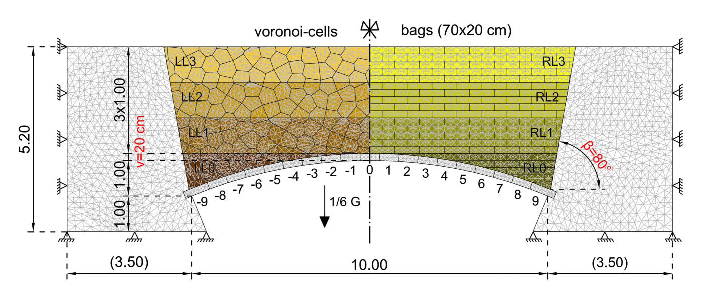
\includegraphics[width=.75\textwidth]{bags.eps}   
      \end{center}  


\end{frame}

\begin{frame}{Temperature dampening due to regolith layers }
For a temperature on the surface, $z = 0$, varied with time,
\begin{align*}
\theta(0,t) & = \theta_{avg}+\theta_0 cos(\omega t)
\end{align*} 
Where $\theta_0$ is half the difference between the high and low temperatures, and $\theta_{avg}$ is the average of the high and low.
 
\end{frame}


  
\begin{frame}{Temperature dampening due to regolith layers }
As layers of regolith insulation surrounding the habitat increase less heat is diffused to the structure.  
We can find the characteristic penetration depth from the thermal diffusivity and omega,
\begin{align*}
\delta & = \sqrt{\frac{D_t}{\omega}}
\end{align*}
Where $D_t = \frac{K_t}{C_v}$

\end{frame}



  
\begin{frame}{Temperature dampening due to regolith layers }
We now have a function of depth and time to use for temperature pulse analysis of the regolith,
\begin{align*}
\theta(z,t) & = \theta_{avg}+\theta_0 e^{\frac{-z}{\delta}} cos(\omega t- \frac{z}{\delta})
\end{align*}

\end{frame}


\begin{frame}{Temperature Dependent Thermal Conductivity}
The thermal conductivity of the regolith changes with the temperature which we can models as,
\begin{align*}
K_t & = k_c \Bigg [ 1+\chi \bigg ( \frac{T}{350} \bigg )^2  \bigg ]
\end{align*}
where the solid conductivity, $K_c = 9.3\times 10^{-3} \frac{W}{mK}$ and $\chi= 0.073$ and is the ratio of radiative to solid conductivity, these have been chosen in accordance with Vasavada et al.\cite{Vasavada}
\end{frame}


\begin{frame}{Heat Capacity}
The heat capacity is found from the bulk thermal inertia, $I = 0.019 m^2 s^{1/2} \frac{K}{J}$ which is set equal to the inverse root of the thermal conductivity, density, and heat capacity \cite{Racca}. 
\begin{align*}
I & = \frac{1}{\sqrt{K_t \rho C_v}} \quad \text{Solving for $C_v$	}\\
C_v & = \frac{1}{K_t \rho I^2}
\end{align*}
Where we tale the density of the regolith to be $ 1900 \frac{Kg}{m^3} $ \cite{Malla}.
\end{frame}

\begin{frame}{Matlab Functions}
We can use Matlab to generate numerical values for the thermal conductivity, which are used to find the heat capacity from the thermal inertial and density where we can then find the penetration depth. A Temperature pulse can then be simulated.
\end{frame}

\begin{frame}{Unprocessed Regolith}
The the top layer of lunar regolith is decribed as a 'fluff' layer that comprises the top 2cm of the surface and has a lower thermal conductivity than the denser lower layers\cite{Malla}.
 \begin{center}
             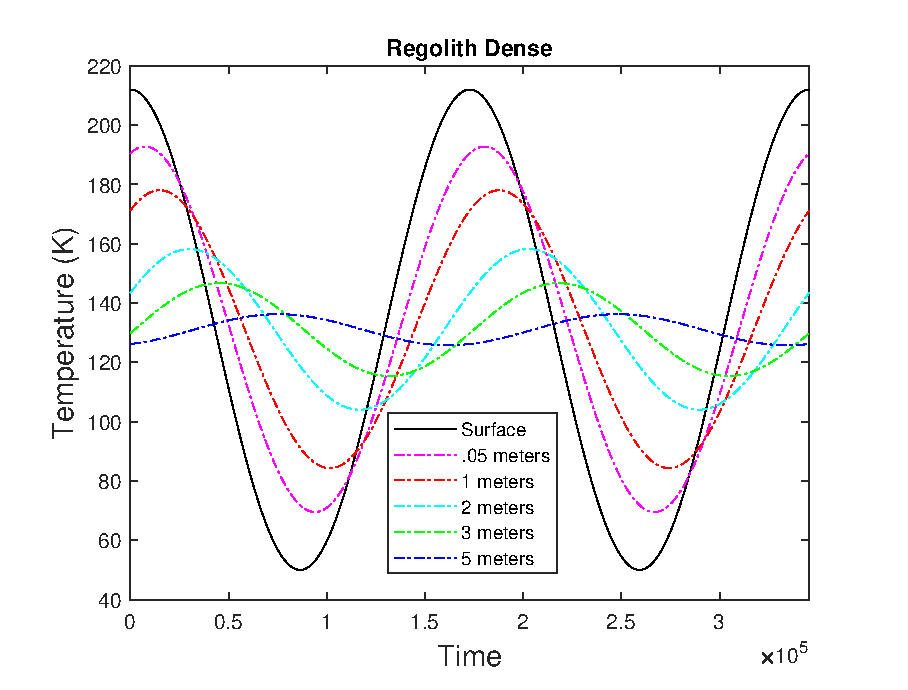
\includegraphics[width= .75\textwidth]{Regolith_Pulse.eps}   
      \end{center}  
\end{frame}


\begin{frame}{Processed Regolith}
Research has shown that by using a loose mixture of the top 'fluff' layer of lunar regolith  which has a lower thermal conductivity and thus higher thermal shielding can be used as a strong insulator\cite{Malla}.
 \begin{center}
             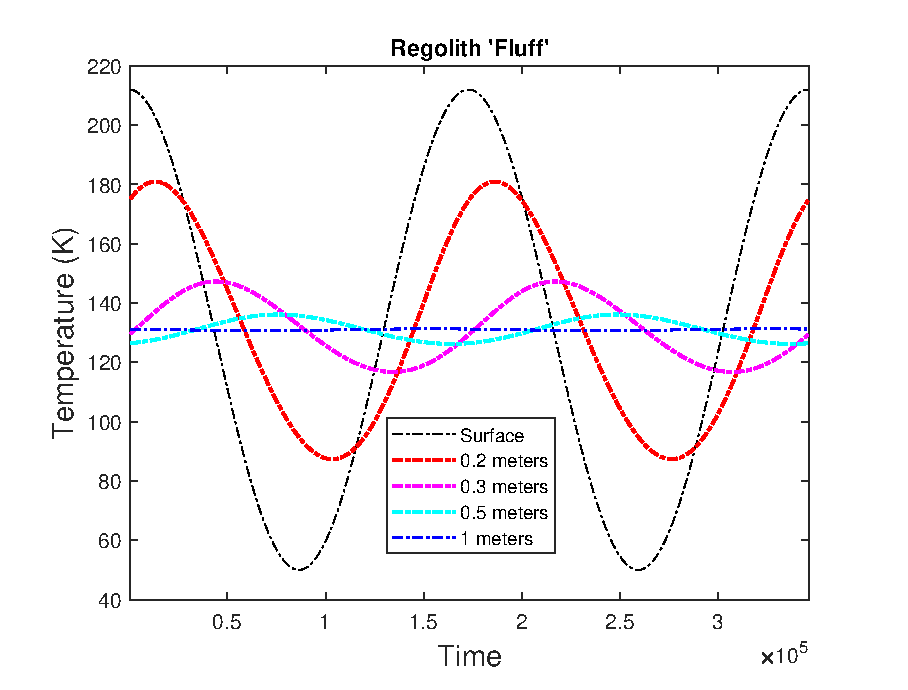
\includegraphics[width= .75\textwidth]{Processed_Regolith.eps}   
      \end{center}  
\end{frame}

\begin{thebibliography}{99}
% The numeral (here 99) in curly braces is nominally the number of entries in
% the bibliography. It's supposed to affect the amount of space around the
% numerical labels, so only the number of digits should matter--and even that
% seems to make no discernible difference.



\bibitem{Koebel}David Koebel, Michele Bonerba, Daniel Behrenwaldt, Matthias Wieser, Carsten Borowy,
Analysis of landing site attributes for future missions targeting the rim of the lunar South Pole Aitken basin,
Acta Astronautica,
Volume 80,
2012,
Pages 197-215

\bibitem{Yao}Xiaochen Lu, Wei Yao, Chao Wang, Rong Ma,
Exergy analysis of a lunar based solar thermal power system with finite-time thermodynamics,
Energy Procedia,
Volume 158,
2019,
Pages 792-796


\bibitem{Belz} Belz et al., 2011. Hybrid life support systems with integrated fuel cells and photobioreactors for a lunar base. Aerospace Science and Technology, pp.Aerospace Science and Technology.

\bibitem{Hickman}Hickman, J.M., Curtis, H.B. \& Landis, G., 1990. Design considerations for lunar base photovoltaic power systems, Washington, DC] : [Springfield, Va.]: National Aeronautics and Space Administration

\bibitem{Climent}Blai Climent, Oscar Torroba, Ricard González-Cinca, Narayanan Ramachandran, Michael D. Griffin,
Heat storage and electricity generation in the Moon during the lunar night,
Acta Astronautica,
Volume 93,
2014,
Pages 352-358

\bibitem{Heldmann}Jennifer L. Heldmann, et al. Site selection and traverse planning to support a lunar polar rover mission: A case study at Haworth Crater,
Acta Astronautica, Volume 127, 2016, Pages 308-320,

\bibitem{Toth}Toth, A.R. \& Bagi, K., 2011. Analysis of a Lunar Base Structure Using the Discrete-Element Method. Journal Of Aerospace Engineering, 24(3), pp.397–401.

\bibitem{Williams}J.P. Williams, D.A. Paige, B.T. Greenhagen, E. Sefton-Nash,
The global surface temperatures of the Moon as measured by the Diviner Lunar Radiometer Experiment,
Icarus,
Volume 283,
2017,
Pages 300-325


\bibitem{Vasavada}A.R.Vasavada,D.A.Paige,S.E.Wood,Near surface temperatures on
mercury and the moon and the stability of polar ice deposits,Icarus
141(1999)179–193.

\bibitem{Racca}G. Racca,Moon surface thermal characteristics for moon orbiting
spacecraft thermal analysis,Planet.SpaceSci.43(1983)835–842.

\bibitem{Malla}Ramesh B. Malla, Kevin M. Brown,
Determination of temperature variation on lunar surface and subsurface for habitat analysis and design,
Acta Astronautica,
Volume 107,
2015,
Pages 196-207

\end{thebibliography}


\end{document}